


\part*{Implementation - Architecture}
\addcontentsline{toc}{chapter}{Architecture}

  \begin{center}
    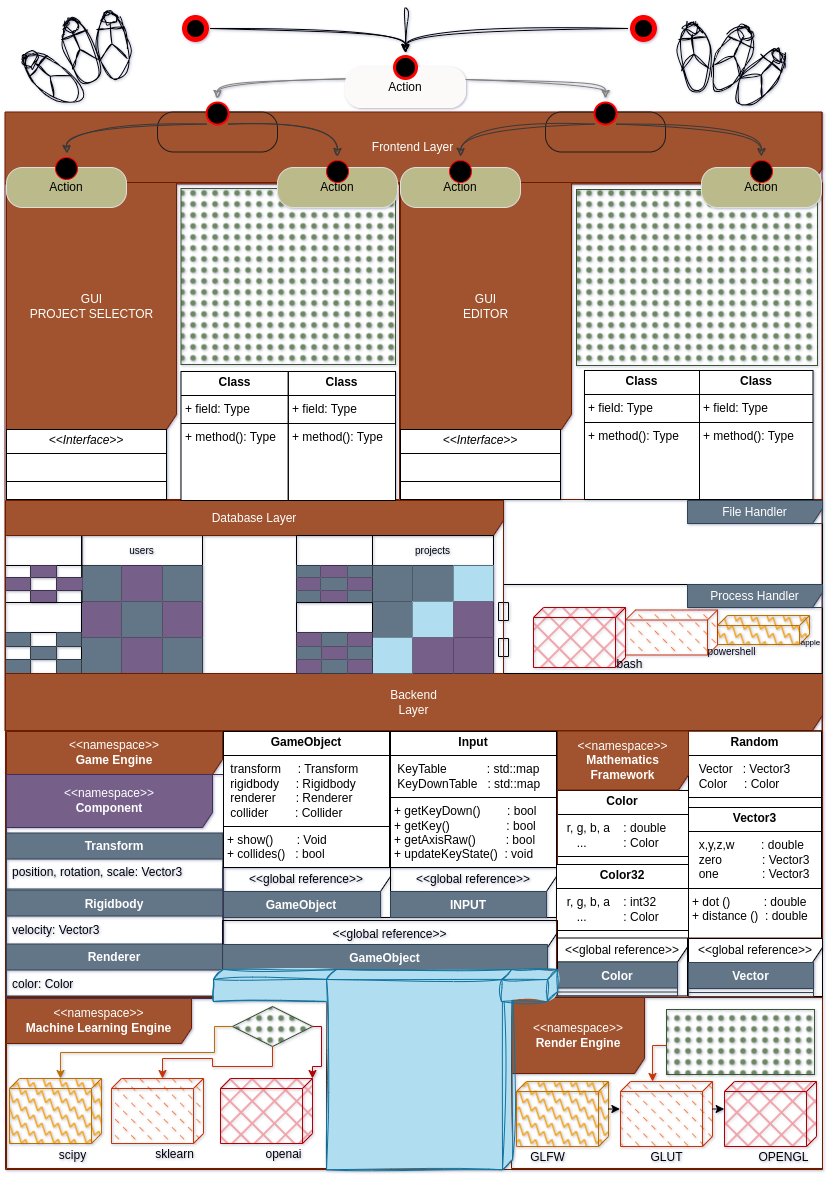
\includegraphics[width=\textwidth]{implementation_arch.png}
  \end{center}
  \pagebreak

  I intent for this project to become a collection of technologies that can be interconnected.
Similar to how Internet-of-Things solutions involve different running parts for achieving one goal, 
as such i want my software making environment to be as versatile as possible. 

  One obvious start impediment is going past the first couple of hello-world projects
  until you find a tool that does the job.

  The percentage of availability of one component can be determined by the color of one's title. 

    \textcolor {red} {bright  colors} means more relevant to this  \textcolor {orange} {iteration}.

    \textcolor {brown} {neutral colors} suggests the component's state of integrity and integration.

    \textcolor {gray} {non-colors} and you're looking at a component that hasn't been integrated yet.

  Future expansion possibilities are in \textcolor {white} {white} color. 


  \begin{itemize}
    \item  \textcolor {brown} { \textbf { FrontEnd ( PyQt   GUI programming interface)} } \\
    \textcolor {gray}   { integration dispatch layer  }
    \item \textcolor {red}    { Backend  ( Python Machine Learning Interface) } \\
      \textcolor {gray}   { communication socket }
    \item \textcolor {orange} { \textbf { Backend  ( C/C++  Render Engine,Math Engine) } }

    \textcolor {white}  { ROBOTICS / ARDUINO / PIE integration }
    % \item \textcolor {gray}   { FrontEnd ( web app ) }
    % \hline \textcolor {gray}   { integration dispatch layer  }
    % \item \textcolor {brown}  { Backend  ( Python Django ) }
    % \item \textcolor {gray}   { Database ( MariaDB) }
\end{itemize}



\pagebreak



\part*{The backend}

  There are two main languages used in this backend implementation:

  \hline
  \hspace{10}

  in C/C++  we have: Rendering Engine, Vectorial MathEngine, GameEngine.

  in Python we have: pyqt editor, Bash File Manager, Machine Learning Interface, Django.

  \chapter*{The Vectorial Math Engine}
  
\section*{Mathematical Framework with Homogenous Representation Support}

Intuitively, for storing a 3D point one might think about using a vector of length 3 ( maybe call them x, y, z ) and have a great day.
Well, this datastructure is good \emph{enough} for most cases.
There is, of course, one little edge-case in one of those cases where we might be needing a fancier solution.
Also, this fancy solution somewhat simplifies the other calculations as well.


This new datastructure implies using a k+1 dimentional vector space for representing k dimensional entities. 

% TODO:  REFERENCE HERE
Meaning that, in our application's purposes, a Vector3 class should store 4 elements. [More about this in future work]


% #include <iostream>
    % // Constructor with default parameters
% // C++ class definition for Vector2
\begin{lstlisting}
class Vector3 
{
  public:
    double x, y, z, w;
    Vector3(double _x, double _y = 0, double _z = 0, double _w = 1) 
           : x(_x), y(_y), z(_z), w(_w) { }
};
\end{lstlisting}


\begin{equation*}
    \mathbf{v_1} = \begin{pmatrix} x_1 & y_1 & z_1 & w_1 \end{pmatrix}.
\end{equation*}

\begin{equation*}
    \mathbf{v_2} = \begin{pmatrix} x_2 & y_2 & z_2 & w_2 \end{pmatrix}.
\end{equation*}





% int main() {
%     // Example usage of Vector3 class
%     Vector3 v1(1.0, 2.0, 3.0);
%     Vector3 v2(4.0, 5.0);

%     std::cout << "v1: (" << v1.getX() << ", " << v1.getY() << ", " << v1.getZ() << ", " << v1.getW() << ")" << std::endl;
%     std::cout << "v2: (" << v2.getX() << ", " << v2.getY() << ", " << v2.getZ() << ", " << v2.getW() << ")" << std::endl;

%     return 0;
% }


% we must be able to do with this DataStructure that would benefit of storing a 3D point as a 4D Vector (x, y, z, \textbf{\emph{w}}).


% This mathematical framework is very important because it assures that the phigs requirements can be fulfiled and how.


\pagebreak

\section*{Please do not be afraid of the \emph{w}.}

  \begin{equation}
    \emph{v.w} =
    \[ \begin{cases} 
      1 & ,\text{if v is used for describing a \hspace{8} point in space}\\ 
      % v ==Vector3::Point\\
      0 & ,\text{if v is used for describing an arrow in space} 
          % ,x::TYPE==Vector3::Arrow
       \end{cases}
    \]
    \label{}
  \end{equation}



Since \emph{w} is defined by a pretty straight-forward formula and the vector \textbf{usually} behaves like a point:


\begin{lstlisting}
    Vector3 v = new Vector3::one * 7
    Debug::Log(v); // <7,7,7,1>
\end{lstlisting}





% TODO: MATH FORMULA FOR w = 1, if point w = 0, if arrow

\section*{Data Structures}
\textbf{Vector Multiplication:}

\begin{equation}
    \mathbf{v_1} \cdot \mathbf{v_2} = (x_1 x_2) + (y_1 y_2) + (z_1 z_2) + (w_1 w_2)
\end{equation}

\textbf{Dot Product of Vectors:}

The dot product \( \mathbf{v}_1 \cdot \mathbf{v}_2 \) between vectors \( \mathbf{v}_1 \) and \( \mathbf{v}_2 \) is calculated as:

\[
\mathbf{v}_1 \cdot \mathbf{v}_2 = v_{1,1} \cdot v_{2,1} + v_{1,2} \cdot v_{2,2} + \cdots + v_{1,m} \cdot v_{2,m}
\]


\textbf{Constructing a Matrix from Vectors:}

Let \( \mathbf{v}_1 = (v_{1,1}, v_{1,2}, \ldots, v_{1,m}) \) be a vector representing the row elements.

Let \( \mathbf{v}_2 = (v_{2,1}, v_{2,2}, \ldots, v_{2,n}) \) be a vector representing the column elements.


\begin{lstlisting}
  v1 = Random::Vector3();
  v2 = Random::Vector3();
\end{lstlisting}


  % matrix = line.dot(column);

  % return matrix;



The resulting matrix \( \mathbf{M} \) formed by these vectors is:

\[
\mathbf{M} = \begin{pmatrix}
v_{1,1} & v_{1,2} & \cdots & v_{1,m} \\
v_{2,1} & v_{2,2} & \cdots & v_{2,m} \\
\end{pmatrix}
\]



  % \subsection*{Matrix Multiplication}
  % \begin{equation}
  %     \mathbf{A} = \begin{pmatrix}
  %     a_{11} & a_{12} & a_{13} & a_{14} \\
  %     a_{21} & a_{22} & a_{23} & a_{24} \\
  %     a_{31} & a_{32} & a_{33} & a_{34} \\
  %     a_{41} & a_{42} & a_{43} & a_{44}
  %     \end{pmatrix}
  % \end{equation}

  % \begin{equation}
  %     \mathbf{B} = \begin{pmatrix}
  %     b_{11} & b_{12} & b_{13} & b_{14} \\
  %     b_{21} & b_{22} & b_{23} & b_{24} \\
  %     b_{31} & b_{32} & b_{33} & b_{34} \\
  %     b_{41} & b_{42} & b_{43} & b_{44}
  %     \end{pmatrix}
  % \end{equation}

  % \begin{equation}
  %     \mathbf{C} = \mathbf{A} \times \mathbf{B} = \begin{pmatrix}
  %     c_{11} & c_{12} & c_{13} & c_{14} \\
  %     c_{21} & c_{22} & c_{23} & c_{24} \\
  %     c_{31} & c_{32} & c_{33} & c_{34} \\
  %     c_{41} & c_{42} & c_{43} & c_{44}
  %     \end{pmatrix}
  % \end{equation}


\pagebreak



\textbf{Matrix Multiplication (Traditional):}
\begin{equation}
    C = A \times B \quad \text{where} \quad C_{ij} = \sum_{k=1}^{n} A_{ik} \cdot B_{kj}
\end{equation}

% \begin{equation*}
%     c_{ij} = \sum_{k=0}^{4} v_{ik} v_{kj} = v_{i1}v_{1j} + v_{i2}v_{2j} + v_{i3}v_{3j} + v_{i4}v_{4j}
% \end{equation*}


\textbf{Strassen Matrix Multiplication (Recursive):}
\begin{equation}
    \mathbf{M}_1 = (A_{11} + A_{22})(B_{11} + B_{22})
\end{equation}
\begin{equation}
    \mathbf{M}_2 = (A_{21} + A_{22})B_{11}
\end{equation}
\begin{equation}
    \mathbf{M}_3 = A_{11}(B_{12} - B_{22})
\end{equation}
\begin{equation}
    \mathbf{M}_4 = A_{22}(B_{21} - B_{11})
\end{equation}
\begin{equation}
    \mathbf{M}_5 = (A_{11} + A_{12})B_{22}
\end{equation}
\begin{equation}
    \mathbf{M}_6 = (A_{21} - A_{11})(B_{11} + B_{12})
\end{equation}
\begin{equation}
    \mathbf{M}_7 = (A_{12} - A_{22})(B_{21} + B_{22})
\end{equation}


\section*{Software Engineering}

There are two main coordinate systems:

\textbf{Cartesian Coordinates:}
\begin{equation}
    (x, y, z)
\end{equation}

\textbf{Polar Coordinates:}
\begin{equation}
    (r, \theta, \phi)
\end{equation}

\textbf{Transformation Formulas:}
\begin{align}
    r &= \sqrt{x^2 + y^2 + z^2} \\
    \theta &= \arctan\left(\frac{y}{x}\right) \\
    \phi &= \arccos\left(\frac{z}{r}\right)
\end{align}







% LATE TODO 
% \begin{itemize}
%   \item Cartesian Coordinates
%   \item Polar     Coordinates 
% \end{itemize}

% Formulas for converting from one to another:
% \begin{itemize}
%   \item from Polar     to Cartesian
%   \begin{itemize}
%     \item cos(x)
%     \item sin(x)
%   \end{itemize}
%   \item from Cartesian to Polar
%   \begin{itemize}
%     \item x
%     \item y
%   \end{itemize}
% \end{itemize}


\pagebreak

In the following, we will take a look over the possible operation that are extensively used:

\textbf{Operations in Computer Graphics}

\textbf{Translation:}
\begin{equation}
    T(x, y, z) = \begin{pmatrix}
    1 & 0 & 0 & x \\
    0 & 1 & 0 & y \\
    0 & 0 & 1 & z \\
    0 & 0 & 0 & 1
    \end{pmatrix}
\end{equation}

\textbf{Scaling:}
\begin{equation}
    S(s_x, s_y, s_z) = \begin{pmatrix}
    s_x & 0 & 0 & 0 \\
    0 & s_y & 0 & 0 \\
    0 & 0 & s_z & 0 \\
    0 & 0 & 0 & 1
    \end{pmatrix}
\end{equation}



These equasions must be really easy to use. 
For this i have chosen the option that highly resembles Unity's ecosystem.


\begin{lstlisting}
void start();
void update();
int main() { Awake(); }
void Awake() {
  RenderEngine::setStart(start);
  RenderEngine::setUpdate(update);
  RenderEngine::setFixedUpdate(fixedUpdate);
  // MUST BE CALLED LAST
  RenderEngine::START(true);
}
void start() {
  Gameobject go; int speed = 0.01;
  Debug::Log(go.transform.name)
  Debug::Log(go.transform.position)
  
  go.transform.translate(Vector3::Right * speed)
  Debug::Log(go.transform.position)
  go.transform.position = Vector3::one * Math::sqrt(Math::pi);
  Debug::Log(go.transform.position)
}
\end{lstlisting}

The implementation feels self-explanatory from here. But for reference i advise 
\href{https://www.github.com}{source-code}





\pagebreak


Here lives the little inconvenience i mentioned at the beginning of the chapter 
that justified Homogenous Coordinates.

\textbf{Rotation with Euler Angles (XYZ order):}
\begin{equation}
    R_{XYZ}(\alpha, \beta, \gamma) = R_X(\alpha) \cdot R_Y(\beta) \cdot R_Z(\gamma)
\end{equation}
where
\begin{align}
    R_X(\alpha) &= \begin{pmatrix}
    1 & 0 & 0 & 0 \\
    0 & \cos\alpha & -\sin\alpha & 0 \\
    0 & \sin\alpha & \cos\alpha & 0 \\
    0 & 0 & 0 & 1
    \end{pmatrix}, \\
    R_Y(\beta) &= \begin{pmatrix}
    \cos\beta & 0 & \sin\beta & 0 \\
    0 & 1 & 0 & 0 \\
    -\sin\beta & 0 & \cos\beta & 0 \\
    0 & 0 & 0 & 1
    \end{pmatrix}, \\
    R_Z(\gamma) &= \begin{pmatrix}
    \cos\gamma & -\sin\gamma & 0 & 0 \\
    \sin\gamma & \cos\gamma & 0 & 0 \\
    0 & 0 & 1 & 0 \\
    0 & 0 & 0 & 1
    \end{pmatrix}
\end{align}

\textbf{Gimbal Lock Issue:} Euler angles suffer from gimbal lock, where two of the three rotational axes align, leading to a loss of one degree of freedom.

\textbf{Solution: Quaternions}
\begin{equation}
    q = \cos\left(\frac{\theta}{2}\right) + \sin\left(\frac{\theta}{2}\right)(u_x i + u_y j + u_z k)
\end{equation}
where \( \theta \) is the rotation angle and \( (u_x, u_y, u_z) \) is the unit vector representing the axis of rotation.




% In most of the cases, the equasions are really easy.

% \subsection*{Translation}
% \subsection*{Scalation}
% \subsection*{Rotation}
% \subsubsection*{Euler-Lock}
% And it would've been all so easy if it weren't for you! 

% Euler Lock is a problem that ocurs when we try to use euler coordinates in rotation aplications. This problem can become extremily dangerous when solving robotics solutions where you can't afford to ???

% \subsubsection*{Quaternions}
% For eliminating the euler-lock problem, quaternions are used. Quaternions are ??

% Formulas:









  \chapter*{The opengl Rendering Framework}
  
\section*{Color32}


\begin{lstlisting}
class color32
{
  public:
    unsigned int r, g, b, a;

    color32(double grayscale) 
           : color(grayscale, grayscale, grayscale, 1.0f) { }
    color32(double _r, double _g, double _b, double _a = 1.0f) {  }
};
\end{lstlisting}




As you can see, similar to the vector class, the color datastructure is also a 4D vector. This will come in handy when dealing with shaders. 


  \subsection*{Opposite Colors}
  \begin{lstlisting}
  class color32
  {
    public:
      unsigned int r, g, b, a;

      color32(double grayscale) 
             : color(grayscale, grayscale, grayscale, 1.0f) { }
      color32(double _r, double _g, double _b, double _a = 1.0f) {  }
  };



  \end{lstlisting}


  \begin{lstlisting}
  void start();
  void update();
  int main() { Awake(); }
  void Awake() {
    RenderEngine::setStart(start);
    RenderEngine::setUpdate(update);
    RenderEngine::setFixedUpdate(fixedUpdate);
    // MUST BE CALLED LAST
    RenderEngine::START(true);
  }
  void start() {
    Gameobject go;
    go.transform.position = Random::Vector3().normalised *  Random::Value(-5, 5); 
    Debug::Log(go.transform.position)
  }
  \end{lstlisting}


\section*{Primitives}

% PHIGS (Programmer's Hierarchical Interactive Graphics System) provides the function:

\begin{lstlisting}

  point(x, y, c); // Changes the color of the pixel at location <x, y> to c

  line(<<x>, <y>>, 
       <<x>, <y>>); // Draws a line between 2 points

  background(color);

  square(point1, point2);
  fill(color);
  circle(point , radius);

  noStroke();
\end{lstlisting}

% \begin{equation}
  % P(x, y), \forall x, y, -\frac{\text{screen::WIDTH}}{2} \leq x \leq \frac{\text{screen::WIDTH}}{2}
  % \label{eq:pixel}
% \end{equation}

These functions are the fundamental building blocks for rendering graphics on a screen in OpenGL. 
For the existance of these functions, 
OpenGL implements various procedures to draw shapes and perform graphical operations.

\subsection*{Points and Lines}

Points and lines are basic graphical primitives. A point is represented by its coordinates \((x, y)\) on the screen, and a line is represented by a linear equation.

\subsubsection*{Line-Drawing Procedure}

A line can be represented by the equation:

\begin{equation}
  y = mx + b
\end{equation}

where \( m \) is the slope of the line, calculated as:

\begin{equation}
  m = \frac{\Delta y}{\Delta x}
\end{equation}

% % ### DDA Algorithm (Digital Differential Analyzer)

% The DDA algorithm is an incremental method for drawing lines:

% \[
% \begin{align*}
%   \Delta x &= x_1 - x_0 \\
%   \Delta y &= y_1 - y_0 \\
%   \text{If } |\Delta x| > |\Delta y|, &\text{ then } \text{steps} = |\Delta x| \text{ else } \text{steps} = |\Delta y| \\
%   \Delta x_{\text{increment}} &= \frac{\Delta x}{\text{steps}} \\
%   \Delta y_{\text{increment}} &= \frac{\Delta y}{\text{steps}}
% \end{align*}
% \]

% Starting from \((x_0, y_0)\), the algorithm increments the coordinates:

% \[
% \begin{align*}
%   x &= x + \Delta x_{\text{increment}} \\
%   y &= y + \Delta y_{\text{increment}}
% \end{align*}
% \]

% % ### Bresenham's Line Drawing Algorithm

% Bresenham's algorithm uses integer arithmetic for efficient computation:

% \[
% \begin{align*}
%   \Delta x &= x_1 - x_0 \\
%   \Delta y &= y_1 - y_0 \\
%   \text{Decision parameter} \, p &= 2\Delta y - \Delta x
% \end{align*}
% \]

% For each \(x\) from \(x_0\) to \(x_1\):

% \[
% \begin{align*}
%   \text{If } p < 0, &\text{ then } p = p + 2\Delta y \\
%   \text{else}, &\text{ increment } y \text{ and } p = p + 2(\Delta y - \Delta x)
% \end{align*}
% \]

% % ### Line Attributes

% % #### Width

% Line width can be controlled using a parameter \(w\):

% \begin{equation}
%   \text{LineWidth}(w)
% \end{equation}

% % #### Color

% Color can be specified using RGB values:

% \begin{equation}
%   \text{Color}(r, g, b)
% \end{equation}

% % #### Segments

% A line segment between two points \((x_0, y_0)\) and \((x_1, y_1)\) can be drawn using the above algorithms, with the line attributes applied.

% \subsection*{Circle-generating Algorithms}

% % ### Midpoint Circle Algorithm

% The midpoint circle algorithm efficiently draws circles using the symmetry of circles and incremental calculations:

% \[
% \begin{align*}
%   x &= r, y = 0 \\
%   \text{Decision parameter} \, p &= 1 - r
% \end{align*}
% \]

% For each \(x\) from \(r\) to 0:

% \[
% \begin{align*}
%   \text{If } p < 0, &\text{ then } p = p + 2x + 3 \\
%   \text{else}, &\text{ decrement } y \text{ and } p = p + 2(x - y) + 5
% \end{align*}
% \]

% % ### Parametric Form

% Using the parametric form of a circle:

% \[
% \begin{align*}
%   x &= r \cos \theta \\
%   y &= r \sin \theta
% \end{align*}
% \]

% \subsection*{Flood-Fill Algorithms}

% Flood-fill algorithms fill a contiguous area of pixels with a specified color.

% % ### Boundary Fill Algorithm

% Starting from a seed point \((x, y)\):

% \[
% \begin{align*}
%   \text{If } P(x, y) \neq \text{boundary\_color} \text{ and } P(x, y) \neq \text{fill\_color}, &\text{ then fill } P(x, y) \text{ and apply to neighboring pixels}
% \end{align*}
% \]

% \subsection*{Text Renderer}

% Rendering text involves drawing each character glyph using the above primitives and positioning them appropriately.

% \section*{Conclusion}

% The described primitives and algorithms form the basis of graphical rendering in OpenGL, allowing the creation of complex images from basic elements like points, lines, and circles.













%       % \begin{itemize}
%       %   \item Points and Lines
%       %   \begin{itemize}
%       %     \item Width
%       %     \item Color
%       %     \begin{itemize}
%       %       \item Flood-Fill Algorithms
%       %     \end{itemize}
%       %     \item Segments
%       %   \end{itemize}
%       %   \item Circle-generating Algorithms
%       %   \item Text Renderer
%       % \end{itemize}

%   % \subsubsection*{Operations}
%   %   \begin{itemize}
%   %     \item Matrices
%   %     \begin{itemize}
%   %       \item Homogeneous Representation
%   %       \item Matrix      Multiplication
%   %     \end{itemize}

%   %     \item Basic Transformations
%   %     \begin{itemize}
%   %         \item Translation
%   %         % TODO: ADD EQUASIONS
%   %         \item Rotation
%   %         \begin{itemize}
%   %             \item Euler Method
%   %             \item Euler Problem
%   %             \item Quaternions
%   %             % TODO: EQUASIONS
%   %         \end{itemize}
%   %         \item Scaling
%   %         % TODO: EQUASIONS
%   %     \end{itemize}
%   %     \end{itemize}







% \section*{Game Engine Component}

% \subsection*{Render Engine}

% \begin{verbatim}
% namespace RenderEngine
% {
%     void Enabled(bool state);
 
%     void setStart (void (*func)());
 
%     void setUpdate(void (*func)());
% }
% \end{verbatim}

% The Render Engine namespace includes functions for enabling or disabling the engine, and setting start and update functions. These functions are represented as follows:

% \[
% \text{Enabled}(state) \rightarrow \text{void}
% \]

% \[
% \text{setStart}(\text{func}) \rightarrow \text{void}
% \]

% \[
% \text{setUpdate}(\text{func}) \rightarrow \text{void}
% \]

% Here, \(\text{func}\) is a function pointer that can be assigned to start or update functions for the engine.

% \subsection*{Vector3 Class}

% \begin{verbatim}
% class Vector3
% {
% public:
%   double x, y, z, w;
%   static Vector3 zero;
%   static Vector3 one;

%   Vector3() : Vector3(0, 0, 0, 1) {}
 
%   Vector3(double _x, double _y = 0.0f, double _z = 0.0f, double _w = 1.0f) 
%     : x(_x), y(_y), z(_z), w(_w) {}
 
%   Vector3& operator=(const Vector3& other);
%   Vector3& operator+=(const Vector3& other);
%   Vector3& operator*=(double scalar);
%   Vector3 operator*(double scalar) const;
%   Vector3 operator-(const Vector3& other) const; 
%   Vector3 operator+(const Vector3& other) const; 
%   double dot(const Vector3& other) const;
%   Vector3 operator/(double scalar) const;
% };
% \end{verbatim}

% Vector operations for the Vector3 class can be represented mathematically as follows:

% \[
% \mathbf{v} = \begin{pmatrix} x \\ y \\ z \\ w \end{pmatrix}
% \]

% Addition:
% \[
% \mathbf{v}_1 + \mathbf{v}_2 = \begin{pmatrix} x_1 \\ y_1 \\ z_1 \\ w_1 \end{pmatrix} + \begin{pmatrix} x_2 \\ y_2 \\ z_2 \\ w_2 \end{pmatrix} = \begin{pmatrix} x_1 + x_2 \\ y_1 + y_2 \\ z_1 + z_2 \\ w_1 + w_2 \end{pmatrix}
% \]

% Dot product:
% \[
% \mathbf{v}_1 \cdot \mathbf{v}_2 = x_1 x_2 + y_1 y_2 + z_1 z_2 + w_1 w_2
% \]

% Scalar multiplication:
% \[
% \mathbf{v} \cdot s = \begin{pmatrix} x \\ y \\ z \\ w \end{pmatrix} \cdot s = \begin{pmatrix} sx \\ sy \\ sz \\ sw \end{pmatrix}
% \]

% \subsection*{Color Class}

% \begin{verbatim}
% class Color
% {
% public:
%   float r, g, b, a;
%   /* 4bit color support */
%   static Color black;
%   static Color white;
%   static Color red;
%   static Color green;
%   static Color blue;
%   static Color yellow;
%   static Color cyan;
%   static Color magenta;
%   static Color gray;
%   static Color darkGray;
%   static Color lightGray;
%   static Color darkRed;
%   static Color darkGreen;
%   static Color darkBlue;
%   static Color brown;
%   static Color orange;
 
%   Color(double _value)
%     : Color(_value, _value, _value, 1.0f) {}
 
%   Color(double _r, double _g, double _b)
%     : Color(_r, _g, _b, 1.0f) {}
 
%   Color(double _r, double _g, double _b, double _a)
%     : r(_r), g(_g), b(_b), a(_a) {}
% };
% \end{verbatim}

% Colors in the Color class can be represented mathematically as:

% \[
% \mathbf{c} = \begin{pmatrix} r \\ g \\ b \\ a \end{pmatrix}
% \]

% Where \(r\), \(g\), \(b\), and \(a\) represent the red, green, blue, and alpha (transparency) components of the color, respectively.

% \subsection*{Component Namespace}

% \begin{verbatim}
% namespace Component
% {
%   class Transform
%   {
%     public:
%       Vector3 position; 
%       Vector3 rotation; 
%       Vector3 scale;    
%   };

%   class Rigidbody
%   {
%     public:
%       Vector3 velocity;
%   };

%   class Renderer
%   {
%     public:
%       Color color;
%   };
% }
% \end{verbatim}

% The Component namespace includes classes for Transform, Rigidbody, and Renderer components. Mathematically, these components can be represented as follows:

% \[
% \text{Transform} = \begin{pmatrix} \text{position} \\ \text{rotation} \\ \text{scale} \end{pmatrix}
% \]

% \[
% \text{Rigidbody} = \text{velocity}
% \]

% \[
% \text{Renderer} = \text{color}
% \]

% Where position, rotation, and scale are Vector3 objects, velocity is a Vector3 object, and color is a Color object.

% \subsection*{GameObject Class}

% \begin{verbatim}
% class GameObject
% {
% public:
%   Component::Transform transform;
%   Component::Rigidbody rigidbody;
%   Component::Renderer renderer;

%   GameObject();
% };
% \end{verbatim}

% A GameObject is composed of a Transform, Rigidbody, and Renderer component. This can be represented as:

% \[
% \text{GameObject} = \begin{pmatrix} \text{Transform} \\ \text{Rigidbody} \\ \text{Renderer} \end{pmatrix}
% \]

% Where each component is as defined in the Component namespace, representing the position, rotation, scale, velocity, and color of the GameObject.



  \chapter*{The Machine Learning libraries interface}
  \input{src/sections/mlInterface}



\part*{The Frontend}

  This too, 
  splits into two.

  We have the software application and the web application.

  As of writing this, no demonstrabable movement had been done in the web application department. 
  The team lead suggests building software solutions that can be easily imported into web applications without needing to re-implement. Research had been done into webGL integration and the low-level graphics calls we use from opengl are compatible with webgl as well. 
  There are even resources involving qt and pyqt integration. As of writing this, all of the GUI work had been done in the qt environment.  


    The software frontend is wrote in PyQt,a python wrapper for the industry standard qt.

  \chapter*{PyQt Editor}
    










    % 

  % \chapter*{}

  \section*{Additional Tools}

    Additional tools has been developed already, tools that improves the programmer's workflow.
    Such example is a web scraper for data collecting.
    Docs for each major component.
    \begin{figure}
      \begin{center}
        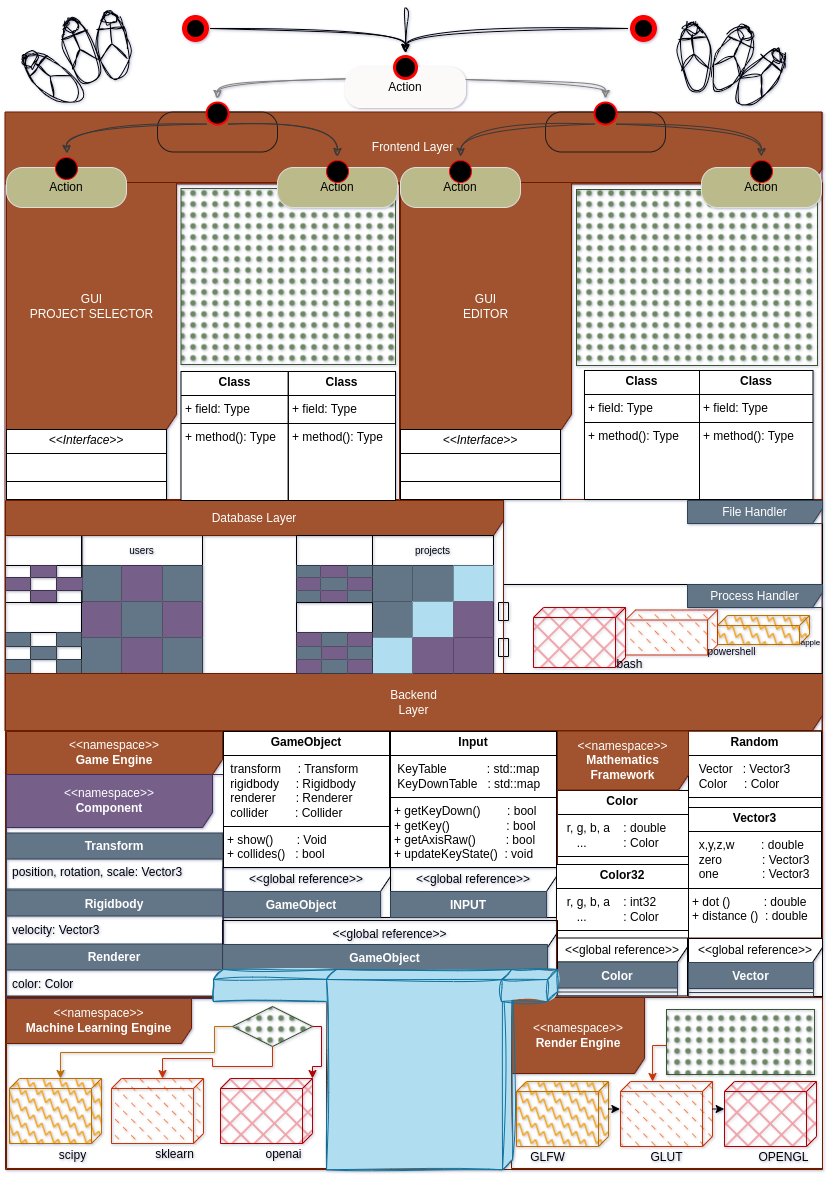
\includegraphics[width=\textwidth]{implementation_arch.png}
      \caption{Arch}
      \end{center}
    \end{figure}

    







    % The software frontend is wrote in PyQt,a python wrapper for the industry standard qt.




\chapter*{pyroGamer - The PyQt Editor}

\section*{Introduction}
The frontend component is called "the PyroGamer project" and is organized into several directories and files. It includes functionalities for the Editor, Hub, and Splash interfaces. These components are managed through various Python scripts and stylesheets. The overall structure can be understood through the following.


\textbf{Directory Structure}

% The directory structure of the frontend is hierarchical. Let \( D \) represent the directory structure where:
\[
  \text{Directory } D := \{d_1, d_2, \ldots, d_n\}
\]
\[
  \text{typeOf} (\( d_i \)) \in \{\text{File}, \text{Directory}\}
\]
% can either be a file or a sub-directory containing further files or sub-directories.

\textbf{Components}

Most of the sub-modules start as this:
\[
F_m = S_m = \{\text{\_\_init\_\_.py}, \text{\_\_main\_\_.py}\}
\]

And then each of them comes with their own required technologies.


% \textbf{\emph{PROJECT LOADER}}

\[
  \text{let hub } H
\xrightarrow{\text{depend}}
\text{cli interface} 
\land 
\text{FileManager} 
\land 
(
\text{gui engine}
\land
\text{icons}
)
% \text{Tabs & Tables}
\]

% \textbf{\emph{Game Editor}}

\[
  \text{let editor } E 
\xrightarrow{\text{depend}}
\text{Hierarchy} 
\land 
\text{SceneView} 
\land 
\text{Inspector}
\land 
(
\text{Assets}
\land 
\text{Terminal}
)
\]

% \subsection*{Editor}
% The Editor component is represented by the set \( E \):
% \[
% E = \{e_1, e_2, \ldots, e_m\}
% \]
% where each \( e_i \) is a sub-directory or file under the Editor directory. Specifically:

\subsubsection*{Configs}
The Configs sub-directory contains scripts for configuration management:
\[
C = \{\text{FileManager.py}, \text{\_\_init\_\_.py}, \text{\_\_main\_\_.py}\}
\]

\begin{lstlisting}[language=Python, caption=FileManager.py]
import os

class FileManager:
    def __init__(self, path):
        self.path = path

    def list_files(self):
        return os.listdir(self.path)
\end{lstlisting}

\subsubsection*{Elements}
The Elements sub-directory is defined as:
\[
L = \{\text{Pages.py}, \text{Tabs}\}
\]
where Tabs itself is a set:
\[
T = \{\text{Assets.py}, \text{Hierarchy.py}, \text{Inspector.py}, \text{SceneView.py}, \text{Terminal.py}\}
\]

\begin{lstlisting}[language=Python, caption=Assets.py]
class AssetsTab:
    def __init__(self):
        self.assets = []

    def add_asset(self, asset):
        self.assets.append(asset)
\end{lstlisting}

\subsubsection*{FileManager and SceneManager}
Both FileManager and SceneManager sub-directories are represented as:
\[
F_m = S_m = \{\text{\_\_init\_\_.py}, \text{\_\_main\_\_.py}\}
\]

\begin{lstlisting}[language=Python, caption=__main__.py]
if __name__ == '__main__':
    print("Initializing Manager")
\end{lstlisting}

\subsubsection*{Styles}
The Styles sub-directory contains CSS files for styling:
\[
S_t = \{\text{createProjWindow.css}, \text{noProjectWindow.css}, \text{projectWindow.css}\}
\]

\subsection*{Hub}
The Hub component is represented by the set \( H \):
\[
H = \{ \text{Configs}, \text{Elements}, \text{icons}, \text{\_\_main\_\_.py} \}
\]

\subsubsection*{Configs}
The Configs sub-directory in Hub contains:
\[
C_h = \{ \text{FileManager.py}, \text{\_\_main\_\_.py} \}
\]

\subsubsection*{Elements}
The Elements sub-directory in Hub is:
\[
L_h = \{ \text{Tables.py}, \text{Tabs.py} \}
\]

\subsection*{Splash}
The Splash component contains:
\[
S_p = \{ \text{images}, \text{\_\_main\_\_.py} \}
\]

\section*{Inter-component Relationships}
The interactions between different components can be represented using functions and mappings. Let \( f: E \to H \) represent the function mapping elements from the Editor to the Hub. Similarly, \( g: H \to S_p \) represents the mapping from Hub to Splash.

\subsection*{File Management}
File management across different components is handled by the scripts in Configs and FileManager directories. Let \( \mathcal{F} \) be the set of file management scripts:
\[
\mathcal{F} = C \cup F_m \cup C_h
\]

\subsection*{Styling}
Styling is governed by CSS files in the Styles directory:
\[
\mathcal{S} = S_t
\]

The overall relationship between these parts can be expressed as:
\[
\text{Frontend} = \mathcal{F} \cup \mathcal{S} \cup (L \cup L_h) \cup S_p
\]

\section*{Conclusion}
The frontend component of PyroGamer is a well-structured combination of directories and files. Each part has a specific role, and their interactions can be mathematically represented to understand the flow and dependencies within the system.







    \pagebreak
